% Use only LaTeX2e, calling the article.cls class and 12-point type.

\documentclass[12pt]{article}

% My packages

\usepackage{graphicx}
\usepackage{amsthm}
\newtheorem{mydef}{Definition}
\usepackage{dcolumn}
\usepackage{multirow}
\usepackage{booktabs}
\newcolumntype{d}{D{.}{.}{4.0}}
\newcolumntype{s}{D{.}{.}{1.4}}

% Users of the {thebibliography} environment or BibTeX should use the
% scicite.sty package, downloadable from *Science* at
% www.sciencemag.org/about/authors/prep/TeX_help/ .
% This package should properly format in-text
% reference calls and reference-list numbers.

\usepackage{scicite}

% Use times if you have the font installed; otherwise, comment out the
% following line.

\usepackage{times}

% The preamble here sets up a lot of new/revised commands and
% environments.  It's annoying, but please do *not* try to strip these
% out into a separate .sty file (which could lead to the loss of some
% information when we convert the file to other formats).  Instead, keep
% them in the preamble of your main LaTeX source file.


% The following parameters seem to provide a reasonable page setup.

\topmargin 0.0cm
\oddsidemargin 0.2cm
\textwidth 16cm 
\textheight 21cm
\footskip 1.0cm


%The next command sets up an environment for the abstract to your paper.

\newenvironment{sciabstract}{%
\begin{quote} \bf}
{\end{quote}}


% If your reference list includes text notes as well as references,
% include the following line; otherwise, comment it out.

\renewcommand\refname{References and Notes}

% The following lines set up an environment for the last note in the
% reference list, which commonly includes acknowledgments of funding,
% help, etc.  It's intended for users of BibTeX or the {thebibliography}
% environment.  Users who are hand-coding their references at the end
% using a list environment such as {enumerate} can simply add another
% item at the end, and it will be numbered automatically.

\newcounter{lastnote}
\newenvironment{scilastnote}{%
\setcounter{lastnote}{\value{enumiv}}%
\addtocounter{lastnote}{+1}%
\begin{list}%
{\arabic{lastnote}.}
{\setlength{\leftmargin}{.22in}}
{\setlength{\labelsep}{.5em}}}
{\end{list}}


% Include your paper's title here

\title{Computational hysteresis:\\ inter-task effects in human computation} 


% Place the author information here.  Please hand-code the contact
% information and notecalls; do *not* use \footnote commands.  Let the
% author contact information appear immediately below the author names
% as shown.  We would also prefer that you don't change the type-size
% settings shown here.

\author
{Edward Newell, Derek Ruths,\\
\\
\normalsize{\texttt{edward.newell@mail.mcgill.ca}}\\
\normalsize{\texttt{druths@networkdynamics.org}}\\
\normalsize{School of computer science, McGill University,}\\
\normalsize{3630 rue University, Montreal, Quebec, H3A 0C6, Canada}\\
\\
}

% Include the date command, but leave its argument blank.

\date{}



%%%%%%%%%%%%%%%%% END OF PREAMBLE %%%%%%%%%%%%%%%%



\begin{document} 

% Double-space the manuscript.

\baselineskip24pt

% Make the title.

\maketitle 



% Place your abstract within the special {sciabstract} environment.

\begin{sciabstract}

Microtask platforms combine the efforts of large numbers 
of people to perform tasks that are difficult to automate with computers 
alone.  These platforms support near-real-time task completion, mimicking a
compute server, and fundamentally shift the role of the human from being a
consumer to being a producer of computing resources.  To realize its full
potential, we must understand how human computation differs from machine 
computation, and in particular address the biases known to be inherent in 
human cognition.  Here we show that when a worker completes a series of 
microtasks, the responses in later tasks are strongly influenced by the 
content of earlier ones.  Our findings are not solely cautionary. We find
evidence that these \textit{inter-task effects} can be
harnessed to improve the quality of responses, and help to achieve 
expert-level judgments, to increase the scope and reliability of citizen 
science and crowdsourcing initiatives.
\end{sciabstract}

\section*{Introduction}
Microtask crowdsourcing platforms like Amazon Mechanical Turk (MTurk) make it 
possible for requesters to submit batches of small tasks to a large pool of 
workers, who do the tasks for fun, a sense of purpose, and remuneration 
\cite{kazai2013analysis,Antin20122925}.  
Originally used to distribute clerical work, these platforms 
increasingly serve as a means to engage experimental 
participants in a research 
setting \cite{paolacci2010running,Berinsky2012351,snow2008cheap,alonso2009can}.
Typical tasks include tagging and categorizing images 
\cite{6116320,Zhai2012357}, transcribing voice recordings 
\cite{chandler2013breaking,paolacci2010running}
or handwritten notes \cite{Berinsky2012351,Finnerty2013}, and judging the 
relevancy of search results \cite{le2010ensuring,grady2010crowdsourcing,alonso2009can,kazai2013analysis}

These platforms make it possible to tightly integrate human and 
machine computation.  Researchers coined the term HPU 
(Human co-Processing Unit) in analogy to CPUs and GPUs \cite{5543192}.  
Ongoing research pursues the establishment of an HPU instruction set
including basic operators like \texttt{vote}, \texttt{subdivide}, \texttt{map},
\texttt{reduce}, \texttt{sentiment}, and \texttt{image\_tag}.  As was 
done with GPU programming, libraries are being developped to give the 
programmer more seamless access to HPU resources 
 \cite{little2010turkit,minder2011crowdlang,minder2012crowdlang,kittur2011crowdforge}.  The availability of human computing platforms makes whole new classes
of problems tractible for the programmer.  For example ***.

But the ability to program with high-level human instructions comes with a 
cost: HPU output is inherently noisy.  Part of this noise could be 
explained by the random differences between workers.  Meanwhile, systematic 
cognitive biases also play a role.  
The phenomenon we attend to here represents yet
another dimension of HPU variance, and arises from the fact that a worker's 
performance changes as a function of the content of previous tasks.  

There has been considerable investigation into the factors that affect the 
output from microtask work.  These include such factors as the 
level of 
pay \cite{kazai2013analysis}, training \cite{le2010ensuring}, pre-screening of 
workers \cite{paolacci2010running}, and user-interface design 
\cite{Finnerty2013}.  Researchers have also investigated \textit{framing}, 
by testing the effects of describing the workflow context 
\cite{Kinnaird2012281}, the purpose of tasks 
\cite{chandler2013breaking}, or using an alternative problem discription
\cite{thibodeau2013natural}.  To our knowledge, no study has investigated 
inter-task effects on microtask platforms.

It is known that people are susceptible to priming effects 
\cite{BJOP1796,No2007,beller1971priming}, and, in particular, task-repetition 
effects \cite{Gass1999549,sohn2001task}.  Thus, a worker's response during
one task may depend in part on previous ones.  Such \textit{inter-task} effects
would amount to a kind of \textit{hysteresis}, meaning that HPU outputs are not
only a function of the current input, but also of the history of inputs, with
important implications for crowdsourcing initiatives.

Here we describe a series of experiments using the Amazon Mechanical
Turk (MTurk) microtask platform that studied inter-task effects
for image-labeling microtasks.  Image-labeling tasks are among the most 
common kinds of microtasks
\cite{chandler2013breaking,Berinsky2012351,Finnerty2013,paolacci2010running}, 
and it seems likely that this will remain the case in the long term because
they provide a source of ground truth in computer vision research 
\cite{5543192}.  
During the experiments, workers performed a series of image labeling tasks, 
and the first five images
they labeled were varied depending on the experimental group to which they
were assigned.  We studied the effects that changing the initial tasks 
had on the labels provided in the final tasks.

As a point of comparison, we included treatments in which we induced
\textit{framing}.
In the framing treatments, before workers begin the tasks, we told them that 
the study was funded by a lab with a particular area of interest, for example,
in the visual perception of food in one case, or the perception of tools in
another.

Surprisingly, inter-task effects were much stronger than framing.  
Our results demonstrate that initial tasks can change 
workers' focus in later tasks.  We also found that inter-task effects altered 
the level of specificity, and the diversity of vocabulary that workers used,
in ways that were not reproduced using framing.
Contrary to our initial expectations, our findings suggest that by carefully
designing workflows, the HPU programmer can leverage inter-task effects to
direct focus, tune specificity, and activate worker expressivity.  Our 
findings carry two lessons for the task designer: inter-task
effects can severely bias HPU output if HPU hysteresis is not taken into 
account, but at the same time, inter-task effects provide another technique
for improving HPU output and may help elicit expert-level annotation.

\paragraph*{Measuring computational hysteresis.}
In setting out to measure the computational hysteresis induced by priming, 
it is important to remember that we are only interested in the practical 
impact of priming on the execution of HPU algorithms.  
The distinction between measuring priming and measuring computational 
hysteresis is subtle, but it is crucial to ensure that our findings are of 
practical significance to crowdsourcing applications.  

This distinction dictates our choice of tools for detecting HPU hysteresis.
A common practice for demonstrating that one population is different from
another (e.g., HPUs exposed to one prime vs another), is to use a 
$\chi^2$ test. This would suffice to demonstrate \textit{whether} priming of 
HPUs had occured, however it says nothing about the \textit{extent} of 
priming, and in particular, does not demonstrate the extent to which primed 
HPUs would execute an algorithm differently.

We opt instead to measure HPU hysteresis using
machine learning algorithms (classifiers), that have been trained to 
distinguish HPUs that were subjected to one prime, from those subjected to 
another.  If a classifier
can distinguish HPUs subjected to different primes, then it serves as 
a kind of certificate, proving 
(up to statistical confidence) that there exists 
an algorithm whose execution is affected by the priming of individual HPUs
(namely, the classifier itself).  This demonstrates that, for some algorithms,
using HPUs primed one way vs another will lead an algorithm to follow a 
different branch of execution with a certain frequency.
Statistically, our approach is grounded in the 
statistical divergence metric called L1-distance 
(alternatively \textit{total variational distance}), via the following 
inequality:
\begin{equation}
	D_\mathrm{L1} \geq 2 \eta - 1, 
	\label{l1}
\end{equation}
where $D_\mathrm{L1}$ is the L1-distance, and $\eta$ is the accuracy of
any binary classifier during validation (provided mild conditions are met). 
Since a classifer's performance estimates
a lower bound on the L1 distance, we shall denote 
$D_\mathrm{L1}^-\equiv 2\eta-1$.
The value of $D_\mathrm{L1}$ ranges from 0 to 1; when $D_\mathrm{L1} = 0$ HPUs 
shown one prime or another are 
indistinguishable, wheras if $D_\mathrm{L1} = 1$ priming is so complete that 
differently primed HPUs can be distinguished perfectly.
The
interested reader will find further discussion of the statistical properties
of our approach and proofs of the above claims in the supplementary material.

\paragraph{Experimental setup.}
We performed two experiments, soliciting respectively 2300, and 900 MTurk 
workers to label images depicting food, kitchen- and dinnerware, and cultural
scenes.  Both experiments had four treatments, and in all treatments of a 
given experiment, the last five ``test'' tasks performed by the workers were 
the same.  Two treatments for each experiment were used to explore inter-task 
effects, by making the initial five tasks for these treatments different.  
For example, in the first 
experiment, the test images depicted clutterd scenes of food and objects,
while ``initial'' images depicted either food only, or non-food objects 
(see Fig. 1).  Although we divide the tasks into initial tasks and test tasks,
no distinction is apparent from the perspective of the worker. Another two 
treatments in both experiments explored framing, 
by presenting the worker with language suggesting a particular research 
intent.  For example, in the first experiment, we stated 
``funded by the laborotary for the visual perception of \{ Objects and Tools 
$\vert$ Food and Ingredients \}''.  For emphasis, the frame text was presented
free of surrounding text, with the variable text in boldface and larger font. 

The experiments and treatments are 
summarized in Table 1, which also introduces short names which we will use to 
identify specific experimental treatments and groupings.
An additional difference between \texttt{exp1} and \texttt{exp2} is that,
in both treatments for \texttt{task1}, workers were shown the test tasks in
one of five permutations, which allows us to analyze the dependance of 
inter-task effects on task proximity, independant of task content.
We provide a fuller account of the experimental design, and exhibit all the
task materials used, in the supplementary material.

\setlength{\tabcolsep}{3pt}
\begin{table}[t]
\centering
\begin{tabular}{ c c c c c }
		\hline \noalign{\smallskip}
		\multicolumn{3}{c}{\textbf{Treatment name}} & \parbox[c]{1.6cm}{\centering \textbf{Framing\\ Prime}} & \parbox[c]{1.7cm}{\centering \textbf{Initial\\ image set}}	\\ 

		\noalign{\smallskip} \hline \noalign{\smallskip}

		\multirow{6}{*}{ \parbox[c]{1cm}{ \phantom{XXX} exp1}} 
			& \multirow{2}{*}{task1} & food & none & food\\
			& & obj & none & objects\\

			\noalign{\smallskip} \cline{2-5} \noalign{\smallskip}
			& \multirow{2}{*}{frame1} & food & food & none\\
			& & obj & objects & none\\

			\noalign{\smallskip} \cline{2-5} \noalign{\smallskip}
			& \multirow{2}{*}{echo} & food & food & none\\
			& & obj & objects & none\\

		\noalign{\smallskip} \hline \noalign{\smallskip}

		\multirow{4}{*}{exp2} 
			& \multirow{2}{*}{task2}  &  food & none & food\\
			& 	&  cult & none & culture\\
			\noalign{\smallskip} \cline{2-5} \noalign{\smallskip}
			& \multirow{2}{*}{frame2} & food & food & food\\
			& 	& cult & culture & food\\

		\noalign{\smallskip} \hline  
	\end{tabular}

	\caption{ \footnotesize{ 
		We use the treatment names shown to refer to specific sections of 
		the data collected.  For example, \texttt{task2:food} refers to the
		treatment in the second experiment which was not exposed to a frame, 
		and whose initial tasks contained images of food (7th row).
	}}
	\label{table:1}
\end{table}

\begin{figure}
	\centering
	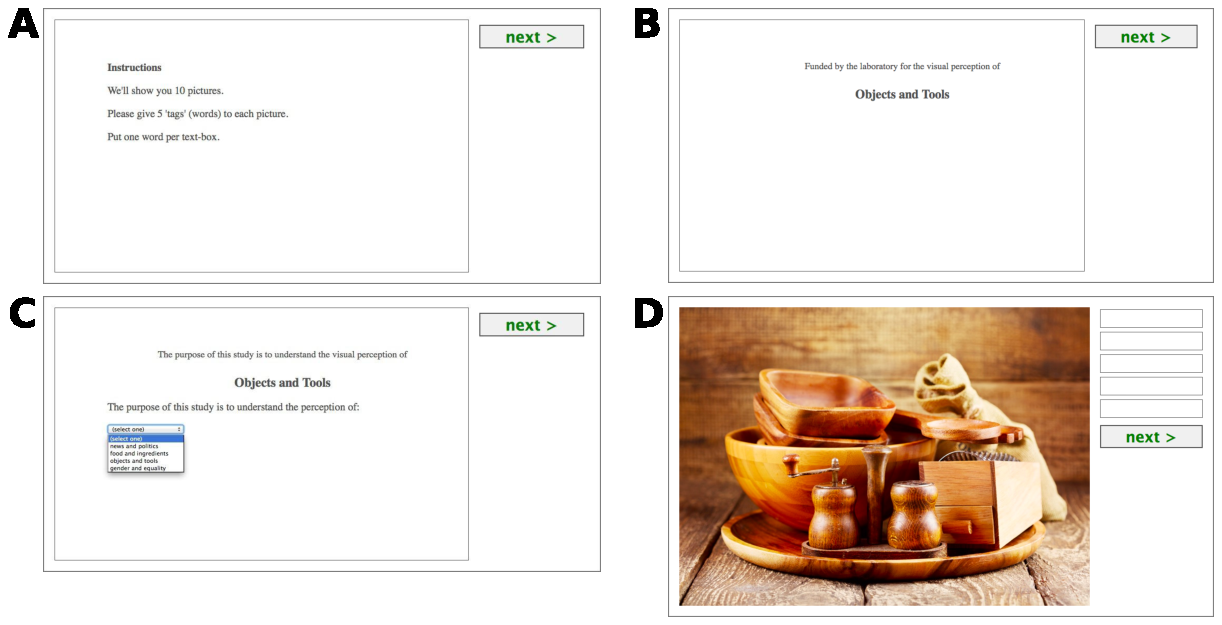
\includegraphics[scale=0.7]{figs/tasks.pdf}
	\caption{Examples of slides used for the image labeling tasks. A) instructions shown to all workers; B) a framing slide; C) a slide from the initial set for treatment IMG:FOOD; D) a slide from the initial set for treatment IMG:OBJ; E) a slide from the test set shown in all treatments. The full set of slides used for all treatments is presented in the supplementary material.}
	\label{fig:task}
\end{figure}


\paragraph{The strength of intertask effects.}

We assessed the strength of intertask and framing effects
by training a multinomial naive Bayes classifier to predict a worker's 
treatment (from two possibilities) based on the labels they provided 
in the test tasks (see Fig.~\ref{fig:theta}).
We found that in \texttt{task1}, whether a worker had labeled food or non-food 
objects during initial tasks, had a strong effect on their subsequent labels, 
biasing them by more than 30\%.  In comparison, the framing effect in \texttt{frame1} did 
not influence workers' labels enough for the classifier predict their treatment
with an accuracy significantly better than chance.  The results for 
\texttt{exp2} show a similar, but even more pronounced trend, with the bias
induced by intertask effects in \texttt{task2} probably exceeding 40\%.

It is worth noting that \texttt{task1} and \texttt{task2} differ in the kind
of comparison that they make.  In \texttt{task1},
the prime concepts (``food'' and ``objects'') are, in certain ways, very 
similar: both are relatively concrete, well-defined concepts, corresponding
to bounded physical entities that can be directly photographed.
But in \texttt{task2}, the prime concepts (``food'' and ``culture''), 
are very different:  culture is far more abstract and difficult to define
than food, and is not a bounded physical entity.  We will come back to this 
point, but note 
here that these pairs of prime concepts both lead to strong intertask effects
despite exploring very different conceptual dimensions.

As another point of comparison, we included additional framing-like 
treatments in \texttt{exp1} in which we attempted to increase the effect.
In the \texttt{echo} treatment pair, we used a more strongly worded frame:
``The purpose of this study is to understand the visual perception of
\{ Objects and Tools $\vert$ Food and Ingredients \}'', and then worker was
asked to reiterate back the purpose of the study, using a combo-box input.
We expected this to induce a strong effect because it signals that this detail
is of particular concern to the task requester, and more important than any of 
the instructions given beforehand.  
The overall effect of these primes was on par with the intertask 
effects in \texttt{task1} (see Fig.~\ref{fig:theta}), which shows just how
powerful intertask effects are.

\begin{figure}
	\centering
	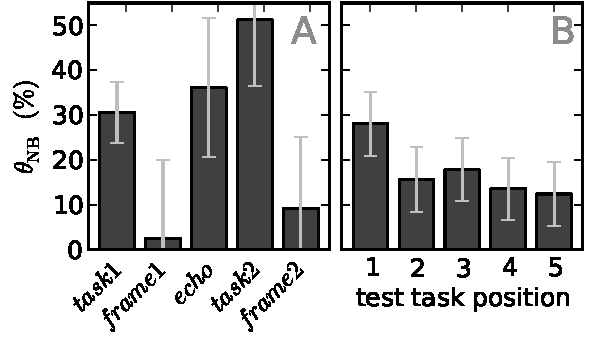
\includegraphics[scale=1]{figs/theta.pdf}
	\caption{
		Difference in priming observed for various pairs of worker populations.
		The pairs of populations differed in terms of the initial tasks they
		performed (bars labeled by \textit{inter-t.}) or in terms of the framing
		to which they were exposed (bars labeled by \textit{frame}; see table 1 for
		details about the treatments).  The difference in priming was 
		measured based on the accuracy of a naive Bayes classifier in 
		resolving which treatment workers belonged to, as described in the 
		text.  
	}
	\label{fig:theta}
\end{figure}

\paragraph{Dynamics of intertask effects.} Following the observation that
intertask effects are strong, it is natural to ask how the effect of an early
task wanes as the worker proceeds through subsequent ones.  To investigate
this, in \texttt{task1} workers performed the test tasks in one of five 
permutations.  This allows us to average the intertask effect accross different
test tasks when they occupy the same position.  We found that the effect was
strongest for the first test image, and that a significant effect persisted
through the five test tasks (see Fig.~\ref{fig:theta}B).  This shows the 
extent to which the first 
test task re-primes workers, washing out the effect of initial tasks, but that
the effect is quite persistent.  In future work, it would be interesting to
investigate whether the first few tasks have a particularly strong priming
effect because they ``set the tone'' for the batch.

This set-up also allows us to see how much the each test tasks differ in their 
susceptibility to intertask effects, independant of their position among the
others.  There does appear to be substantial differences, but relative
position of the test task is more important (Fig.~\ref{fig:theta}C).


\paragraph{Effects on workers' direction of focus} 

Having observed significant effects from framing and task-exposure,
we looked in greater detail at the nature of the effects.  For instance,
does a food-oriented exposure induce workers to provide more food-related
labels?  And if so, does this explain the classifier's ability to distinguish
a worker's initial exposure? 

To answer these questions we used the wordnet corpus, augmented with names of
ethnic foods learned from the Internet.  Wordnet provides a (roughly)
hierarchical set of relationships between nouns, called hypernym-hyponym
relationships.  A hypernym is a generalization, while a hyponym is a 
specialization.  So, for example, ``bread'' is hypernym to ``rye bread'' 
and hyponym to ``baked goods''.

Using the hypernym-hyponyms structure of wordnet to identify nouns depicting
food, we found that, for the experimental pairings in \texttt{exp1}, the
food-exposed treatments did produce a significantly larger fraction of 
food-related labels (see Fig.~\ref{fig:specificity}A).  While the shift in 
focus with regard to food does help explain how workers differ depending on 
their exposure, it still leaves most of this difference unexplained.
Furthermore, in \texttt{exp2:task2} we see a significant but reversed effect
(see Fig.~\ref{fig:specificity}A).
Given the difference between the food-culture and food-object axes, it should
not be surprising that the effect of exposure is different.  This tells us that
the differences induced by exposure to frames or initial tasks are significant,
but would appear to be the result of countervailing influences, with the
overall outcome dependant on the particular axis of the exposures, we will
come back to this momentarily.

To explore these effects further, we looked more closely at which particular
labels are most suppressed (activated) by a workers exposure.  We found that, 
for all treatment pairs, ``food'' was always the most suppressed label among 
the food-exposed workers.  This is surprising, given that we have just seen 
that the bulk incidence of food-related labels \textit{increased} among 
food-exposed workers in most treatment pairs.
Since ``food'' is the most generic food-related word in the wordnet-based
ontology, it follows that food-exposed workers have opted to provide more
specialized references to food rather than using ``food''.

Considerable thought must be given to shaping the the vocabulary with which
a worker engages a task.  To draw an example from the domain of citizen 
science, in galaxy zoo, workers catalogue images of galaxies in terms of
smoothness, rings, dustlanes, digital disturbances, and so on.  Shaping this
vocabulary, is accomplished through a combination of positive and negative
examples during training, peer-to-peer and peer-to-expert engagement in 
discussion areas, and using the interface to constrain and prompt the 
worker.

In our set-up, where the worker's vocabulary is unconstrained, we can 
directly see the effects that frames and initial tasks induce on worker 
vocabulary.
By looking at the number of unique food-related labels that workers 
produced, we assesed the richness of vocabulary that workers used when 
referring to food (see Fig.~\ref{fig:specificity}B.  We found that the 
food-exposed workers use a richer vocabulary of 
food-related words, even in cases like \texttt{task2:food}, where the 
food-exposed treatment made fewer references to food overall.  
Interestingly, in this respect, initial taske exposure had a stronger effect
than framing, including the \texttt{echo} treatment pair. This makes sense, 
given that the various images shown in the initial
tasks would tend to activate a variety of memories and concepts related to 
food, reducing the threshold for later activation during the test-tasks.

Using the ontology of food induced by wordnet, we perform a more detailed
calculation of the relative specificity of workers from different treatments.
To do this, we considered all the labels from one treatment
(for example \texttt{task1:food}) and compared these to all the labels from 
another (\texttt{task1:obj}).  For all possible comparisons, we observed 
which treatment's label was more specific more often.  We normalied this
as a percentage (details in supplementary material) so that we can compare the
relative change in specificity between different treatment pairs  .


Performing the above-mentioned calculation while restricting focus to 
food-related labels (see Fig.~\ref{fig:specificity}C), we found that 
the food-exposed workers always provided food-references of substantially 
greater specificity.  In this respect, the effect induced by 
echoed framing was stronger than that induced by the initial task exposures in
\texttt{task1}.

Taking the all the results shown in Fig.~\ref{fig:specificity} together,
a picture emerges which explains the differing natures of intertask and framing
effects.  First, both negative and positive priming would appear to be at play.
Negative priming occurs when a repeated stimulus, which is perceived to be
nonsalient, begins to be ignored.  As a worker from \texttt{task1:food}
proceeds through the initial tasks, food-related memories and concepts are
activated, reducing increasing the likelihood that she provides a variety of
different food-related labels.  This increases the number of food-related
labels, and increases the richness and specificity of her food-related 
vocabulary.  But meanwhile, in the most general sense, the fact that the 
pictures contain food becomes negatively primed.  She does not regard ``food''
to be a meaningful label, and is inhibited in providing it.   
As for the worker in \texttt{task2}, similar effects occur as she proceeds
through the initial tasks.  Upon viewing the first test task, the introduction
of a very prominent cultural element is novel, and is attended to, whereas
her counterpart in \texttt{task2:cult} has seen several images containing 
cultural themes, and is negatively primed to the general setting of culture,
but responds to the novelty of the introduction of food.  Finally, looking at
the results for \texttt{echo}, we see evidence of its effects operating through
the executive faculties of the worker.  There is considerably more
restriction to food-related labels, and even a greater specificity of such 
labels, but, lacking the diverse activations of food-related memories and 
concepts from initial tasks, the richness of vocabulary is lower.

Based on these observations, we submit several recommendations for the 
consideration for the designers of croudsourced initiatives.
\begin{enumerate}
	\item{
		Examples provide a valuable way to clarify intstructions, but 
		training tasks should be preferred, since they activate concepts and 
		faculties relevant to the subsequent task.
	}
	\item{
		Examples used for training should not be too ``clean'', but should 
		contain the same distribution of noise, or distracting features, as 
		is observed in the real dataset.
		This may help desensitize the worker to the nonsalient features.
		Using training tasks that are too clean will make the subsequent noise
		more novel and thus more distracting.
	}
	\item{
		It is common practice to plant \textit{validation tasks}, for which the
		correct answer is known, to verify worker reliability.
		These tasks should simultaneously be considered as 
		\textit{callibration tasks}, which help
		the worker to maintain an optimally primed state.
		Giving feedback, for both correct and incorrect callibration tasks, 
		may help further reinforce the salient features for the tasks.
	}
	\item{
		Some tasks require the classification of imbalanced datasets.
		For example, in the detection of pre-ictal (pre-siezure) EEG traces,
		the majority of traces are normal.  The absence of exposure to the 
		positive class can lead to a loss of activation for the
		salient features and a drifting conceptualization of the class.
		Using callibration tasks drawn from the underrepresented class may 
		help sustain workers' attention and recall for that class.
	}
	\item{
		When a very precice classification is needed, it may be helpful to
		performing the classification in multiple steps.  For example, in a 
		binary classification, the workers could initially perform a coarse
		classification, using three options for response: 
		``definitely class 0'', ``definitely class 1'', and 
		``borderline''.  Following the coarse classification, the 
		``borderline'' examples could be served in batches together, 
		allowing workers to focus on finer distinctions which are salient 
		in the context of borderline examples.
	}
\end{enumerate}

Each of these techniques can and should be tested directly, and the the
lessons derived from those experiments should be encorporated into the best 
practices for human computation.

\paragraph{Conclusion.}
Our results definitively show that intertask effects can
be as strong as framing effects, and appear in general to be stronger.
Intertask effects have are similar in strength to direct 
statements about the purpose of the tasks, followed by the reiteration of the
purpose by the worker.  However, they differ in the detailed effects that
they bring about.  Initial tasks had a greater effect on richness of 
spontaneously elicited vocabulary used to refer to the primed concept,
whereas the echoed purpose had a somewhat stronger effect increasing the 
quantity of references to the primed concept.

The task designer would do well to give consideration to intetask effects
when performing task batching, and when designing training and validation
tasks.  Despite all efforts to eliminate biases in the microtask setup,
the greatest source of biases may lurk in the tasks themselves.  
But the task designer need not seek to factor out intertask effects altogether.
Rather we advocate regarding intertask effects as a tunable parameter which
can be used to optimize HPU performance.  By correctly directing attention
and conceptual activation, intertask effects may be helpful in exceeding
expert annotations using non-expert HPU computing in a wider variety of
applications.

\paragraph{Effects on label vocabulary and specificity.}
\begin{figure}
	\centering
	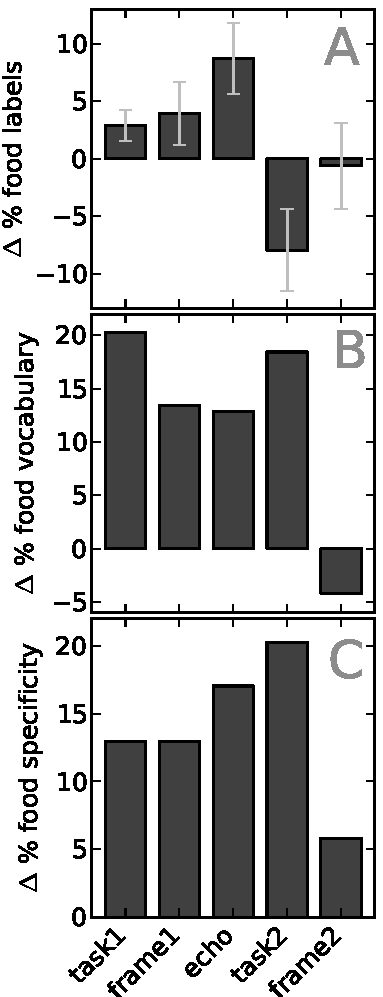
\includegraphics[scale=1]{figs/vocab_specificity.pdf}
	\caption{
		Difference in priming observed for various pairs of worker populations.
		The pairs of populations differed in terms of the initial tasks they
		performed (bars labeled by \textit{inter-t.}) or in terms of the framing
		to which they were exposed (bars labeled by \textit{frame}; see table 1 for
		details about the treatments).  The difference in priming was 
		measured based on the accuracy of a naive Bayes classifier in 
		resolving which treatment workers belonged to, as described in the 
		text.  
	}
	\label{fig:specificity}
\end{figure}

We gain some insight into the induced intertask effects by looking at the
labels whose frequencies changed the most due to workers' early task exposure. 
For example, the ``food'' is the most strongly suppressed label among 
workers exposed to food-related initial tasks.  At first, this may seem 
unexpected, since, for \texttt{task1:food}, food labels are more common 
overall.  But ``food'' is the most generic possible food-related label, 
so this means that \texttt{task1:food} workers are trading their usage of
``food'' for more specific food references.

The richness and specificity of vocabulary that a worker brings to a 
characterization task is of great importance in crowdsourcing.  For example,
in the Galaxy Zoo citizen science project, workers are 
trained to develop a lexicon of galaxy features such as the smoothness,
the presence of rings, dustlanes, digital disturbances, etc.  In our set-up,
the workers lexicon is unconstrained and un-scaffolded, so we can see 
how initial tasks alter the workers lexicon spantaneously.

To investigate this we used the wordnet corpus, which has embeds a rich
nested ontology of concepts in the form of hypernym-hyponym noun relationships.
A hypernym is a generalization, while a hyponym is a specialization; for 
example ``bread'' is a hypernym of ``pumpernickel''.  Using wordnet, we 
can represent the labels produced by one group of workers, for example 
\texttt{task1:food}, and compare it to those labelled by \texttt{taks1:obj}.
We describe the details of this comparison in the supplementary material,
but the result is a net tally of all the cases where a word of the first 
group is more specific than one from the second, less the cases where the 
word of the second group is more specific.

By performing this specificity comparison, while restricting our focus to
food-related words, we can see that workers are in fact induced to be 
significantly more specific in their usage of food-related words (see Fig.XX).


in their usage 
food-related terms in \texttt{task1:food}
than in \texttt{task1:obj}.


one 
to be more specific, less those found to be less specific, in comparing the 
words of the one to those of the other.



citizen science efferts, like galaxy zoo.

food-related labels.
to \textit{more specific} food-labels.


food-related labels are,
overall, 
food-  This is true even when the there are more food-related
terms overall

tasks.  Interestingly, we see that the label ``food'' is always suppressed
in food-primed treatments, but this effect is particularly strong for the


changing initial tasks (and frames) by looking at those labels that show
the greatest frequency change
primes 
When manually inspecting the labels of \textit{test-t.2}, one striking 
observation was that workers that initially labeled images of cultural scenes 
were more likely to use generic words when labeling the test images, compared 
to workers that initially labeled images of meals.  For example, 76\% of the 
workers from \textit{exp2.task.cult} gave the very generic label 
\texttt{food}, compared to only 16\% of \textit{exp2.task.food} workers 
(recall that the test tasks for both treatments depicted prepared meals).
One interpretation is that workers who have already labeled 5 images relating
to food are more likely to focus on aspects of the images that are different
from one another, and refrain from so generic a term as \texttt{food}.

Based on this observation, we tested the degree of specificity of labels 
accross all treatments.  We appraoched measuring specificity in two ways.
Our first method was based on the reasoning that, if a given group of 
workers uses more specific labels, they will then provide, on the whole,
a larger set of unique labels for any given image.  For example,
suppose the workers from \textit{exp2.task.food} who do not use the label 
\texttt{food} had chosen more specific labels instead.  In being more 
specific, they must choose a particular detail to describe, from a large 
number of possibilities, and so are more likely to provide unique labels.
Indeed
for all images in the test set, workers from \textit{exp2.task.food} gave
more unique labels than did those from \textit{exp2.task.cult}, as shown 
in fig 2B.  Note how the the relative vocabulary sizes follows
the same trend, as a function of test task, as was observed for the 
classifier-based detection of general priming differences (c.f. fig X).

Our second approach to measuring relative specificity used the 
hypernym-hyponym relationships of wordnet.
We operationalized the relative specificity of two sets of labels $P$ 
and $Q$ as:
$$
	S(P,Q) = \frac{1}{|P \times Q|}\sum_{p \in P} \sum_{q \in Q} 
		\left(\mathbf{1}_{[p>q]} - \mathbf{1}_{[q>p]}\right),
$$
where $\mathbf{1}_{[p>q]}$ evaluates to 1 if $p$ is a hyponym of $q$.
Using the above equation, we found that, for every images in the 
test set, the labels attributed by workers in \textit{exp2.task.food} were 
more specific than those by workers in \textit{exp2.task.cult}.

Initialy we hypothesized that the similarity of initial and test tasks was
driving a relative increase in specificity.  While this seems reasonable,
we also notice a similar effect occuring for \textit{exp1.task} in which
the test tasks consisted of both food and non-food objects, and the initial
tasks were either food or non-food objects.  In this case, it is difficult
to argue that one set of initial tasks is more similar to another.  In fact
we devise a method to operationalize image similarity, and find that 
the initial images of \textit{exp1.task.food} are equally similar to the
test tasks as the initial images of \textit{exp1.task.obj}.  Furthermore,
we see strong effects on relative specificity for framing as well.

In general, it is of great practical interest to control the level of 
specificity of qualitative characeterzations.  In many applications the
task-designer will probably want obtain characterizations that are more
discriminative.  Thus, when designing microtasks, one should give careful
consideration to inter-task effects.  Unfortunately, we are not sure
why certain initial tasks produced increased specificity as opposed to others, 
and this is a question we intend to pursue in future research.

\paragraph{Conclusions.}
Our results show that inter-task effects can have a strong influence on how 
workers label images. In particular, we observed that prior tasks influence 
the specificity and content of labels. Surprisingly, framing a task by 
indicating a semantically-loaded funder had much milder effects on worker 
outputs, generally below the statistical power of our tests.

We therefore caution those designing studies using human computation: even if 
the requester has eliminated surrounding influences to every practical extent, 
\textit{the greatest source of bias might lurk in the tasks themselves}. Due 
consideration should be given to how tasks are bundled together. While our 
measurements of $\hat{\theta}_\mathrm{NB}$ indicated that inter-task effects 
persisted even to the fifth test image, the most severe effects arise between 
consecutive tasks.

Our proposed priming definition yields general purpose measure of priming 
effects. We used three approaches to detect priming effects: 1) using a Naive 
Bayes classifier to measure $\hat{\theta}_\mathrm{NB}$, 2) tallying the 
number of culture- and food-oriented labels, and 3) comparing the relative
specificity of labels based on an ontology. Of the three, $\theta_\mathrm{NB}$ 
was the most sensitive.

In one sense, this is not surprising because the Naive Bayes classifier takes 
into account the frequency of occurrence of all labels encountered during 
training. But it is remarkable that the method which incorporates neither 
prior knowledge about the image contents nor label semantics, outperforms 
those that do. This is a powerful feature because, given the outputs from two 
sets of workers, one can test whether they have been differently primed 
without knowing how that priming might manifest.

Our algorithmic definition of priming is phrased in terms of worker outputs 
rather than psychological phenomena. This provides a connection between the 
priming effects and their potential to impact decisions made on the basis of 
worker outputs. In the case of a 1-bit binary decision, $\theta$ describes the 
worst-case bias introduced by failing to control for priming effects.

Batching similar tasks together appears to yield higher more specific HPU 
outputs. Our proposed connection between similarity and specificity during 
image-labeling might be used to tune the specificity of labels. For example, 
If one seeks very nuanced labeling, our results suggest that the images 
should first be sorted into batches based on their similarity. This could be 
accomplished by beginning with a first, coarse labeling of unsorted images, 
followed by bundling based on the similarity of coarse labels. Then, bundles 
of similar images could be served for a second round of finer labeling. The 
sorting and re-labeling could in principle be repeated.

Such a workflow involves serial processing, which points to an interesting 
possible differ- ence difference between HPUs and CPUs. In general, whenever 
an aspect of a problem can be parallelized when employing CPUs, one gains 
efficiency. But here, because of HPU hysteresis, one might gain precision by 
using HPUs with a more serialized algorithm. Further testing is needed to 
determine the gain in precision from this approach.


\bibliography{newbib}
\bibliographystyle{Science}


\section*{Supplementary Material}

\subsection*{Assessing task similarity}
\begin{table}
\centering
\begin{tabular}{ l  s s s s}

\toprule    
Image set   
& \multicolumn{1}{c}{Ambig.} 
& \multicolumn{1}{c}{Cultural} 
& \multicolumn{1}{c}{Ingr.}
& \multicolumn{1}{c}{Test} \\
  
\midrule

Ambiguous  & 1 & 0.0418 & 0.142 & 0.167 \\

Cultural  & 0.0418  & 1 & 0.0347 & 0.0561 \\

Ingredients  & 0.142  & 0.0347 & 1 & 0.110 \\

Test & 0.167  & 0.0561 & 0.110 & 1
\\
\bottomrule

\end{tabular}
\caption{\footnotesize{
Pairwise similarities of each image set based on the labels attributed to them (see \textbf{Eq. 4}).
}}
\label{table:2}
\end{table}

One weakness of the above analysis is the reliance on the informal notion
of the similarity of one set of images to another. The 
characterization of image content is a deeply complex issue that has been 
approached by many disciplines \cite{panofsky1939studies,shatford1986analyzing,Tversky1977327,Jaimes20002}. \textit{Perceptual similarity} is a 
particularly recalcitrant concept.   But to formalize our claim, we seek a 
measure of similarity between two sets of images, 
\textit{with respect to the labeling task}.  This can be operationalized
in a straightforward way, by using the similarity of the labels given to images
as a proxy for the similarity of the images.  Thus, to measure the 
similarity between two sets of images, X and Y , we computed the Jacquard 
index between the sets of labels attributed to them:
$$
	\mathrm{Sim}(X,Y) = \frac{L(X) \cap L(Y)}{L(X) \cup L(Y)}
$$
where $L(X)$ denotes the set of labels attributed to images in $X$.

The pairwise similarities of the image sets are presented in Table 2. This 
shows that the workers that yielded higher specificity labels were from 
treatments whose initial tasks were more similar to the test tasks (c.f.
\textbf{Fig 3}).

Such a phenomenon would be consistent with the psychological mechanism known as
\textit{negative priming}.

\end{document}




















%Next we observed how inter-task effects on label composition (i.e. food- vs 
%culture-oriented labels) evolve as workers proceed through test images. We 
%define the excess cultural orientation as the number of culture-oriented 
%labels minus the number of food oriented ones. To meaning- fully compare the 
%excess cultural orientation between test images, we must, however, account 
%for the fact that some images inherently carry more cultural content than 
%others. In keeping with our notion of priming difference, we calculate the 
%excess cultural content for both CULTimg and
%
%AMBG, and take their difference to be the relative excess cultural content, 
%$\Delta_{cult}$. Formally,
%
%		*** Formula for delta cult\ldots
%
%where $N^(i)_{w,cult}$ stands for the number of culture-oriented labels 
%attributed by worker w to image i, while $N^(i)_{w,food}$ similarly counts
%food-oriented labels, and $N$ is the total number of labels in a treatment.
%
%We found $\Delta_{cult}$ was largest for the first test image, but dropped off 
%rapidly, 
%remaining positive but not to a statistically significant extent (see Fig. 3B).
%This is similar to the behavior of $\hat{\theta}_\mathrm{NB}$, however, 
%because the statistical significance of $\Delta_{cult}$ dropped more quickly, 
%$\hat{\theta}_\mathrm{NB}$ appears to be a more sensitive measure of 
%inter-task effects.

